\chapter{Deep feature learning}
\section{Principal Component Analysis}
PCA is a dimensionality reduction technique where data observations of N dimensions  are projected onto a lower dimension space. PCA involves computing the covariance matrix of the normalized input vector which gives the information about the principal components (eigen vectors). These eigen vectors defines the amount of variance in each principal component. In this exercise, we first apply PCA on two different datasets. One is randomly generated Gaussian data of 500 observations and 50 dimensions and the other is choles data with 264 observations and 21 dimensions. The results of PCA on both these data is shown in the figure \ref{fig:Ex_3_1}.\\

\begin{wrapfigure}{L}{0.5\textwidth}
	\captionsetup{format = hang}
	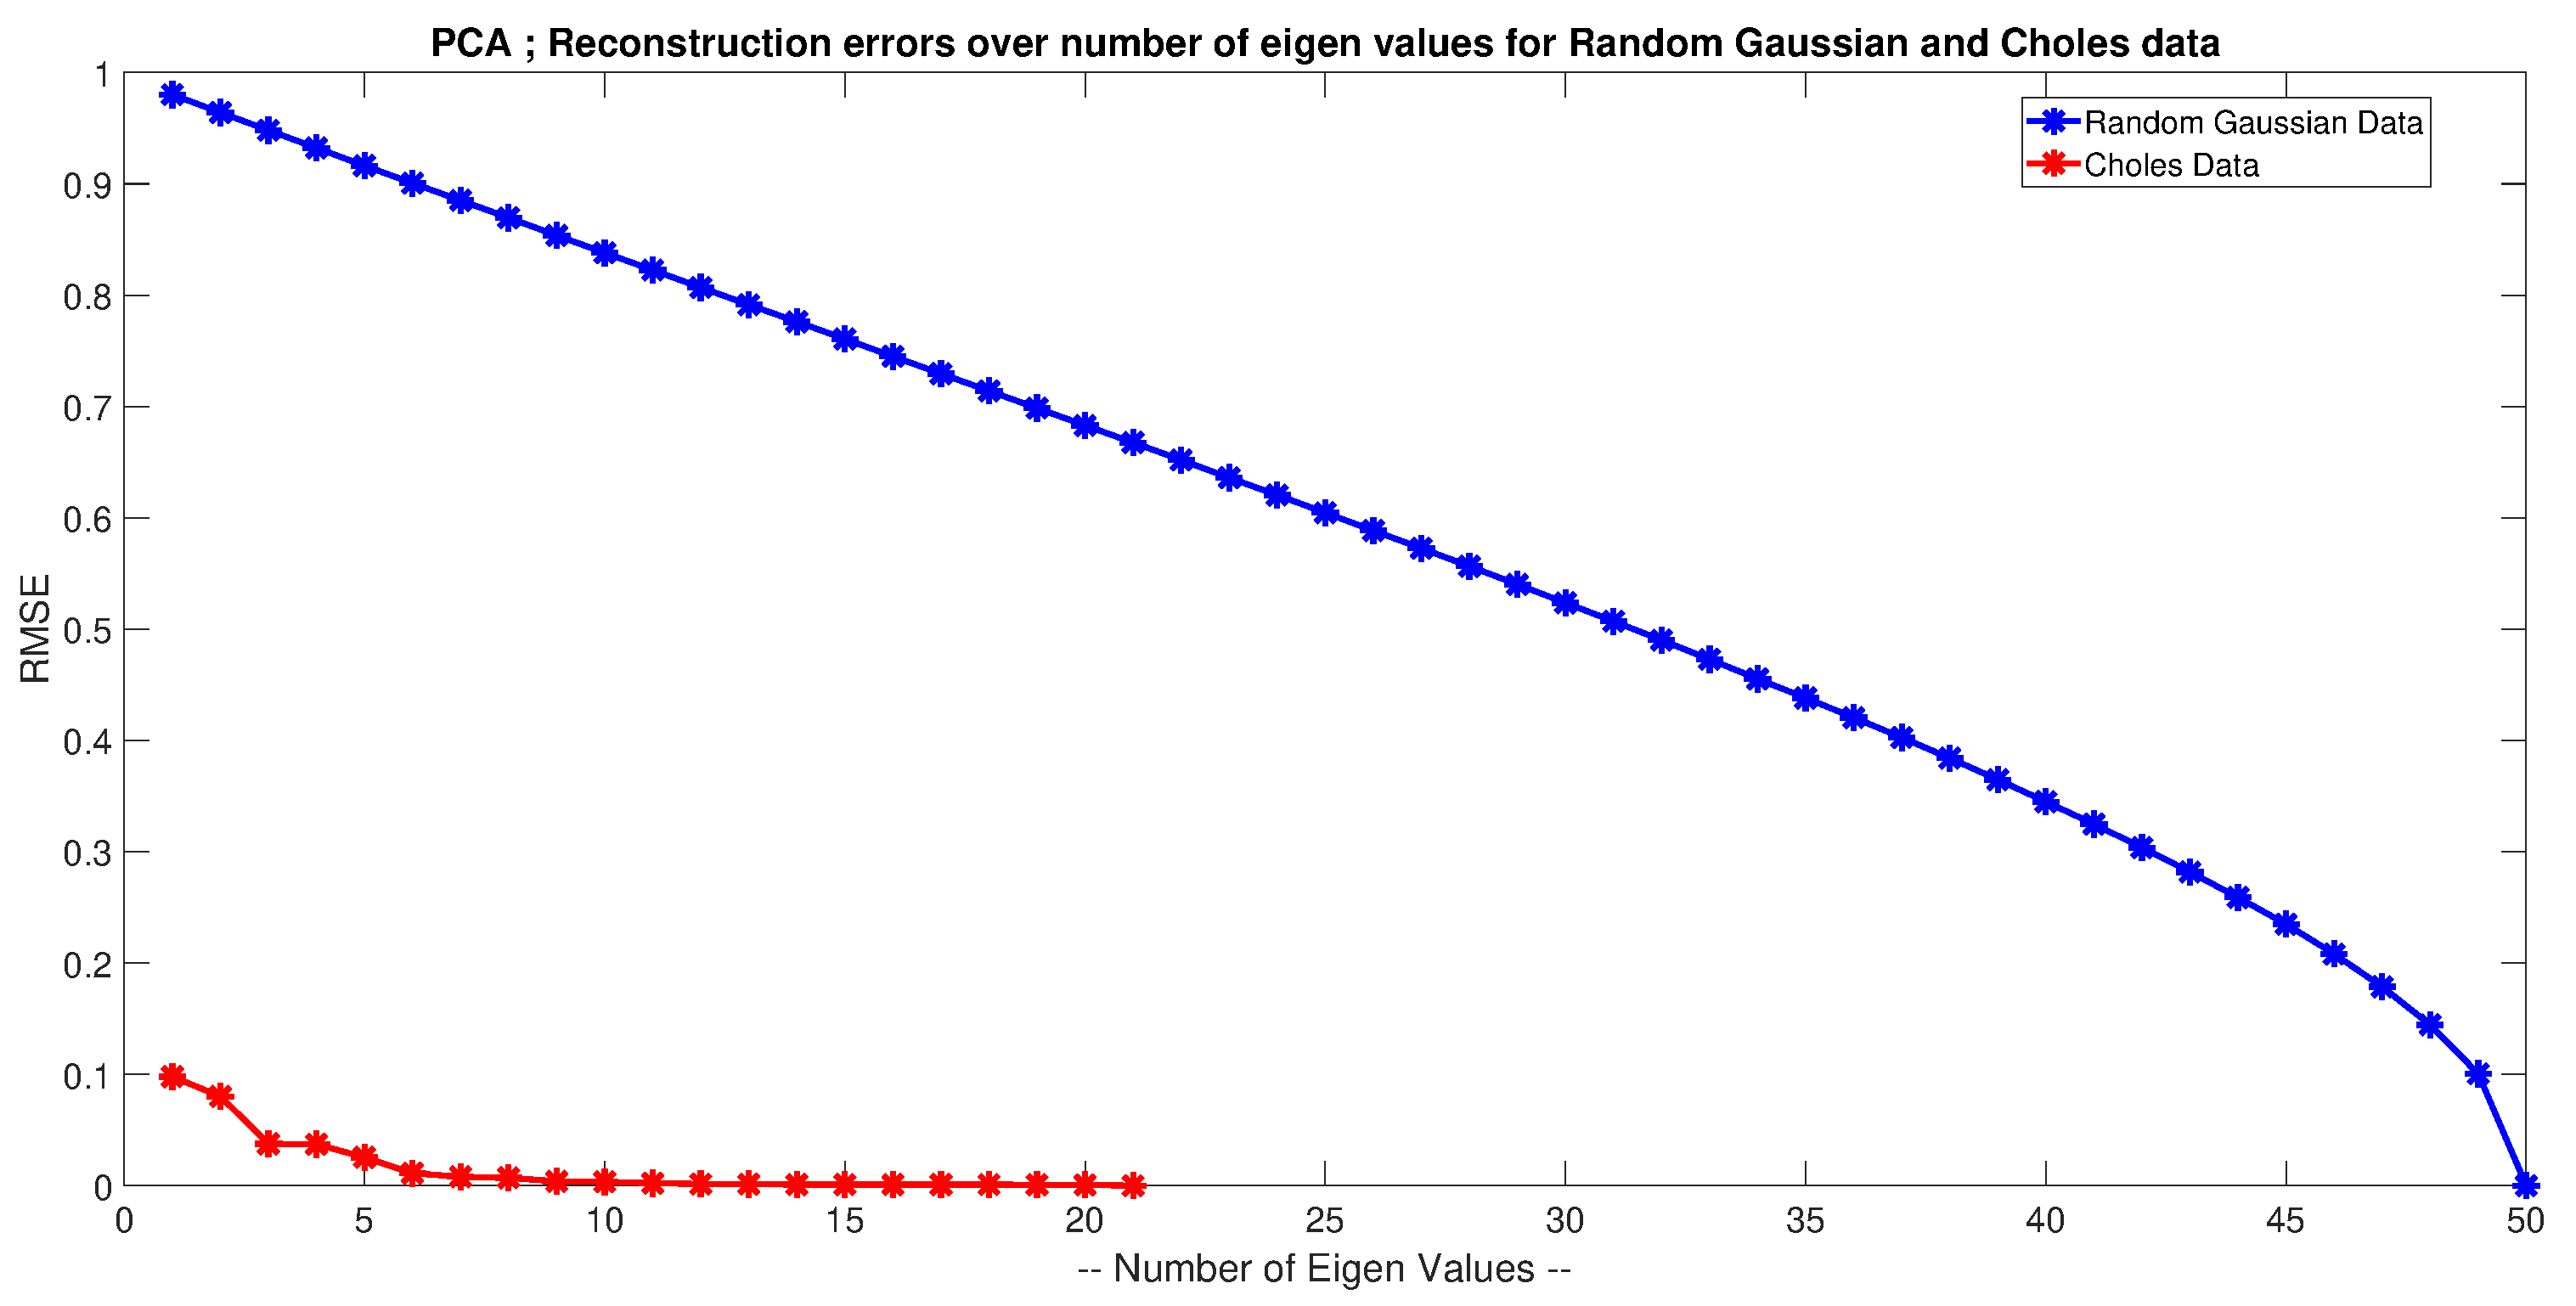
\includegraphics[height = 0.5\textwidth,width = 1\textwidth]{Exercise3/Report/Ex_3_1}
	\caption{PCA on random Gaussian and Choles datasets}\label{fig:Ex_3_1}
\end{wrapfigure}
From the figure \ref{fig:Ex_3_1} it can be noticed that for highly co-related choles data, the reconstruction error is very minimum compared to randomly distributed gaussian data. This is because, the variance among the data observations are very less compared to the random gaussian data. Also, the reconstruction error becomes close to zero after few eigen values for choles data whereas random gaussian data takes 50 which is its original dimensions. We then proceed to perform PCA on handwritten digits dataset of digit 3 for first 4 principal components and then increase the number of principal components upto 256. The results are shown in the below figure \ref{fig:dig3}.
\begin{figure}[!htpb]
	\centering
	\begin{subfigure}[b]{0.5\textwidth}
		\captionsetup{width=0.9\linewidth, format = hang}
		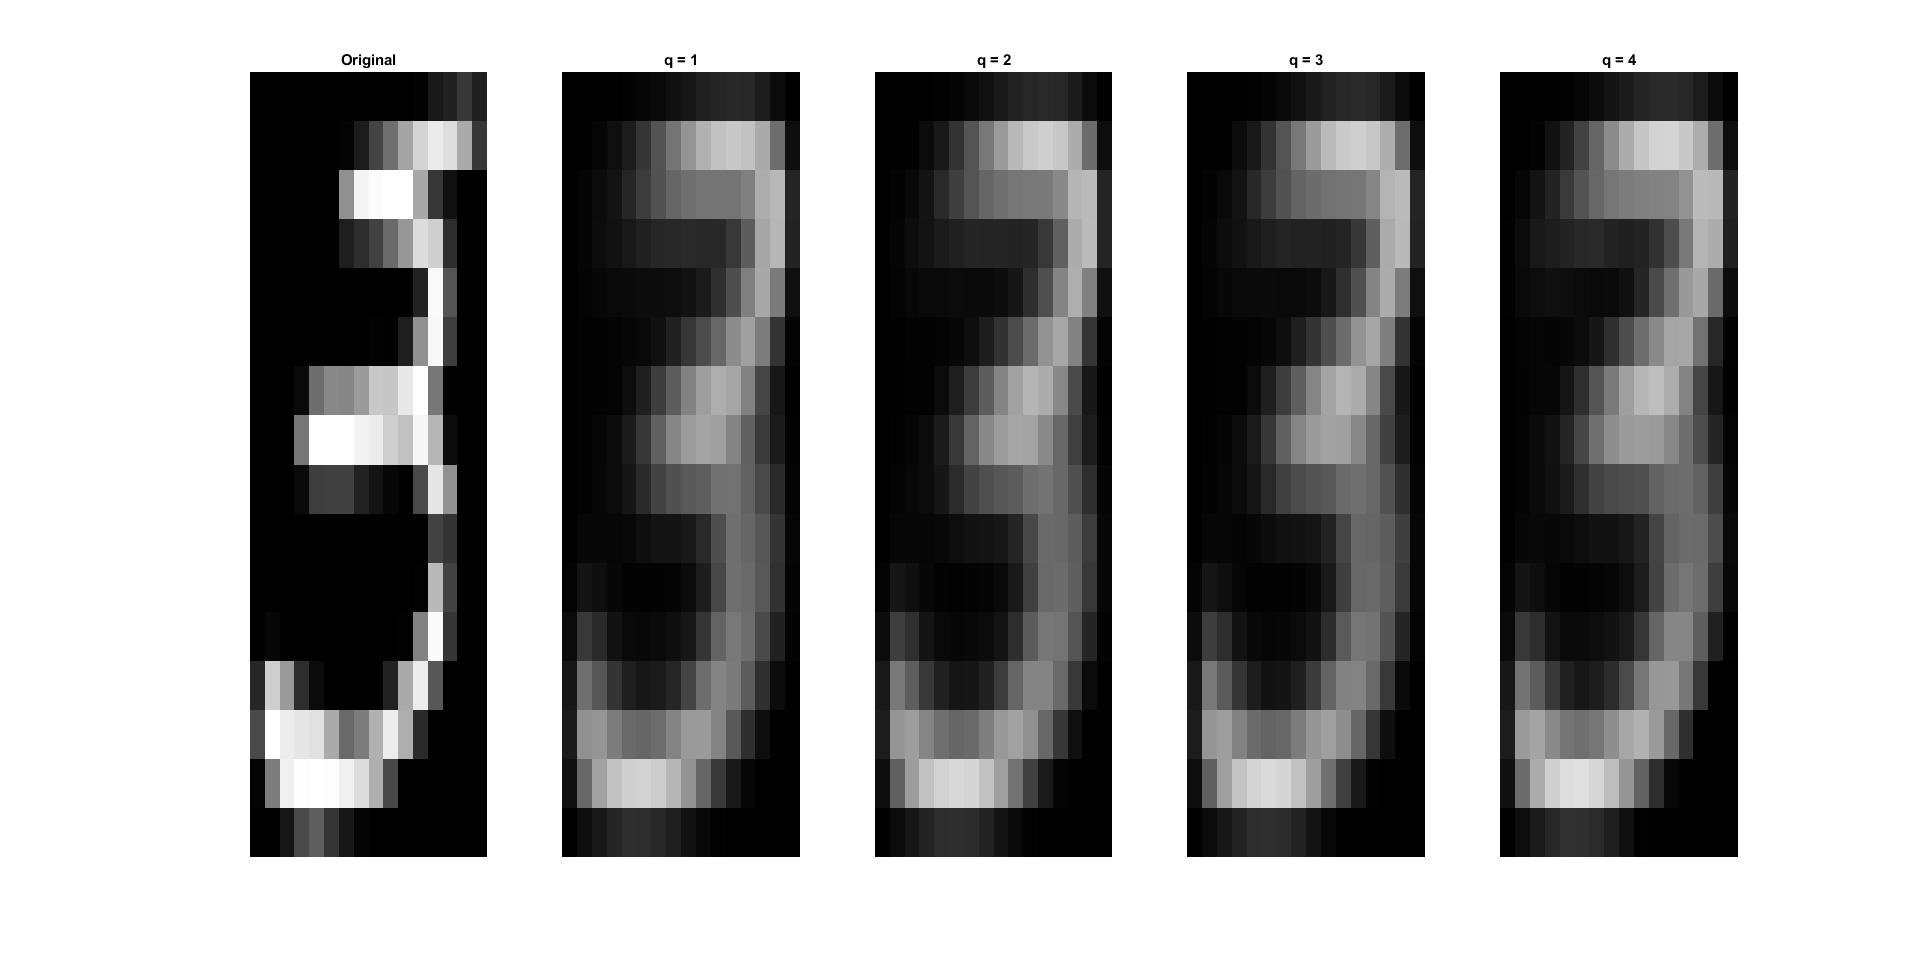
\includegraphics[height = 0.3\textwidth,width = 1.1\textwidth]{Exercise3/Report/pca_dig_1}
		\caption{Original image and reconstructed images with PCA Components [1, 2, 3, 4] - second image to end from left }\label{fig:dig3_1}
	\end{subfigure}%
	\begin{subfigure}[b]{0.5\textwidth}
		\captionsetup{width=0.9\linewidth, format = hang}
		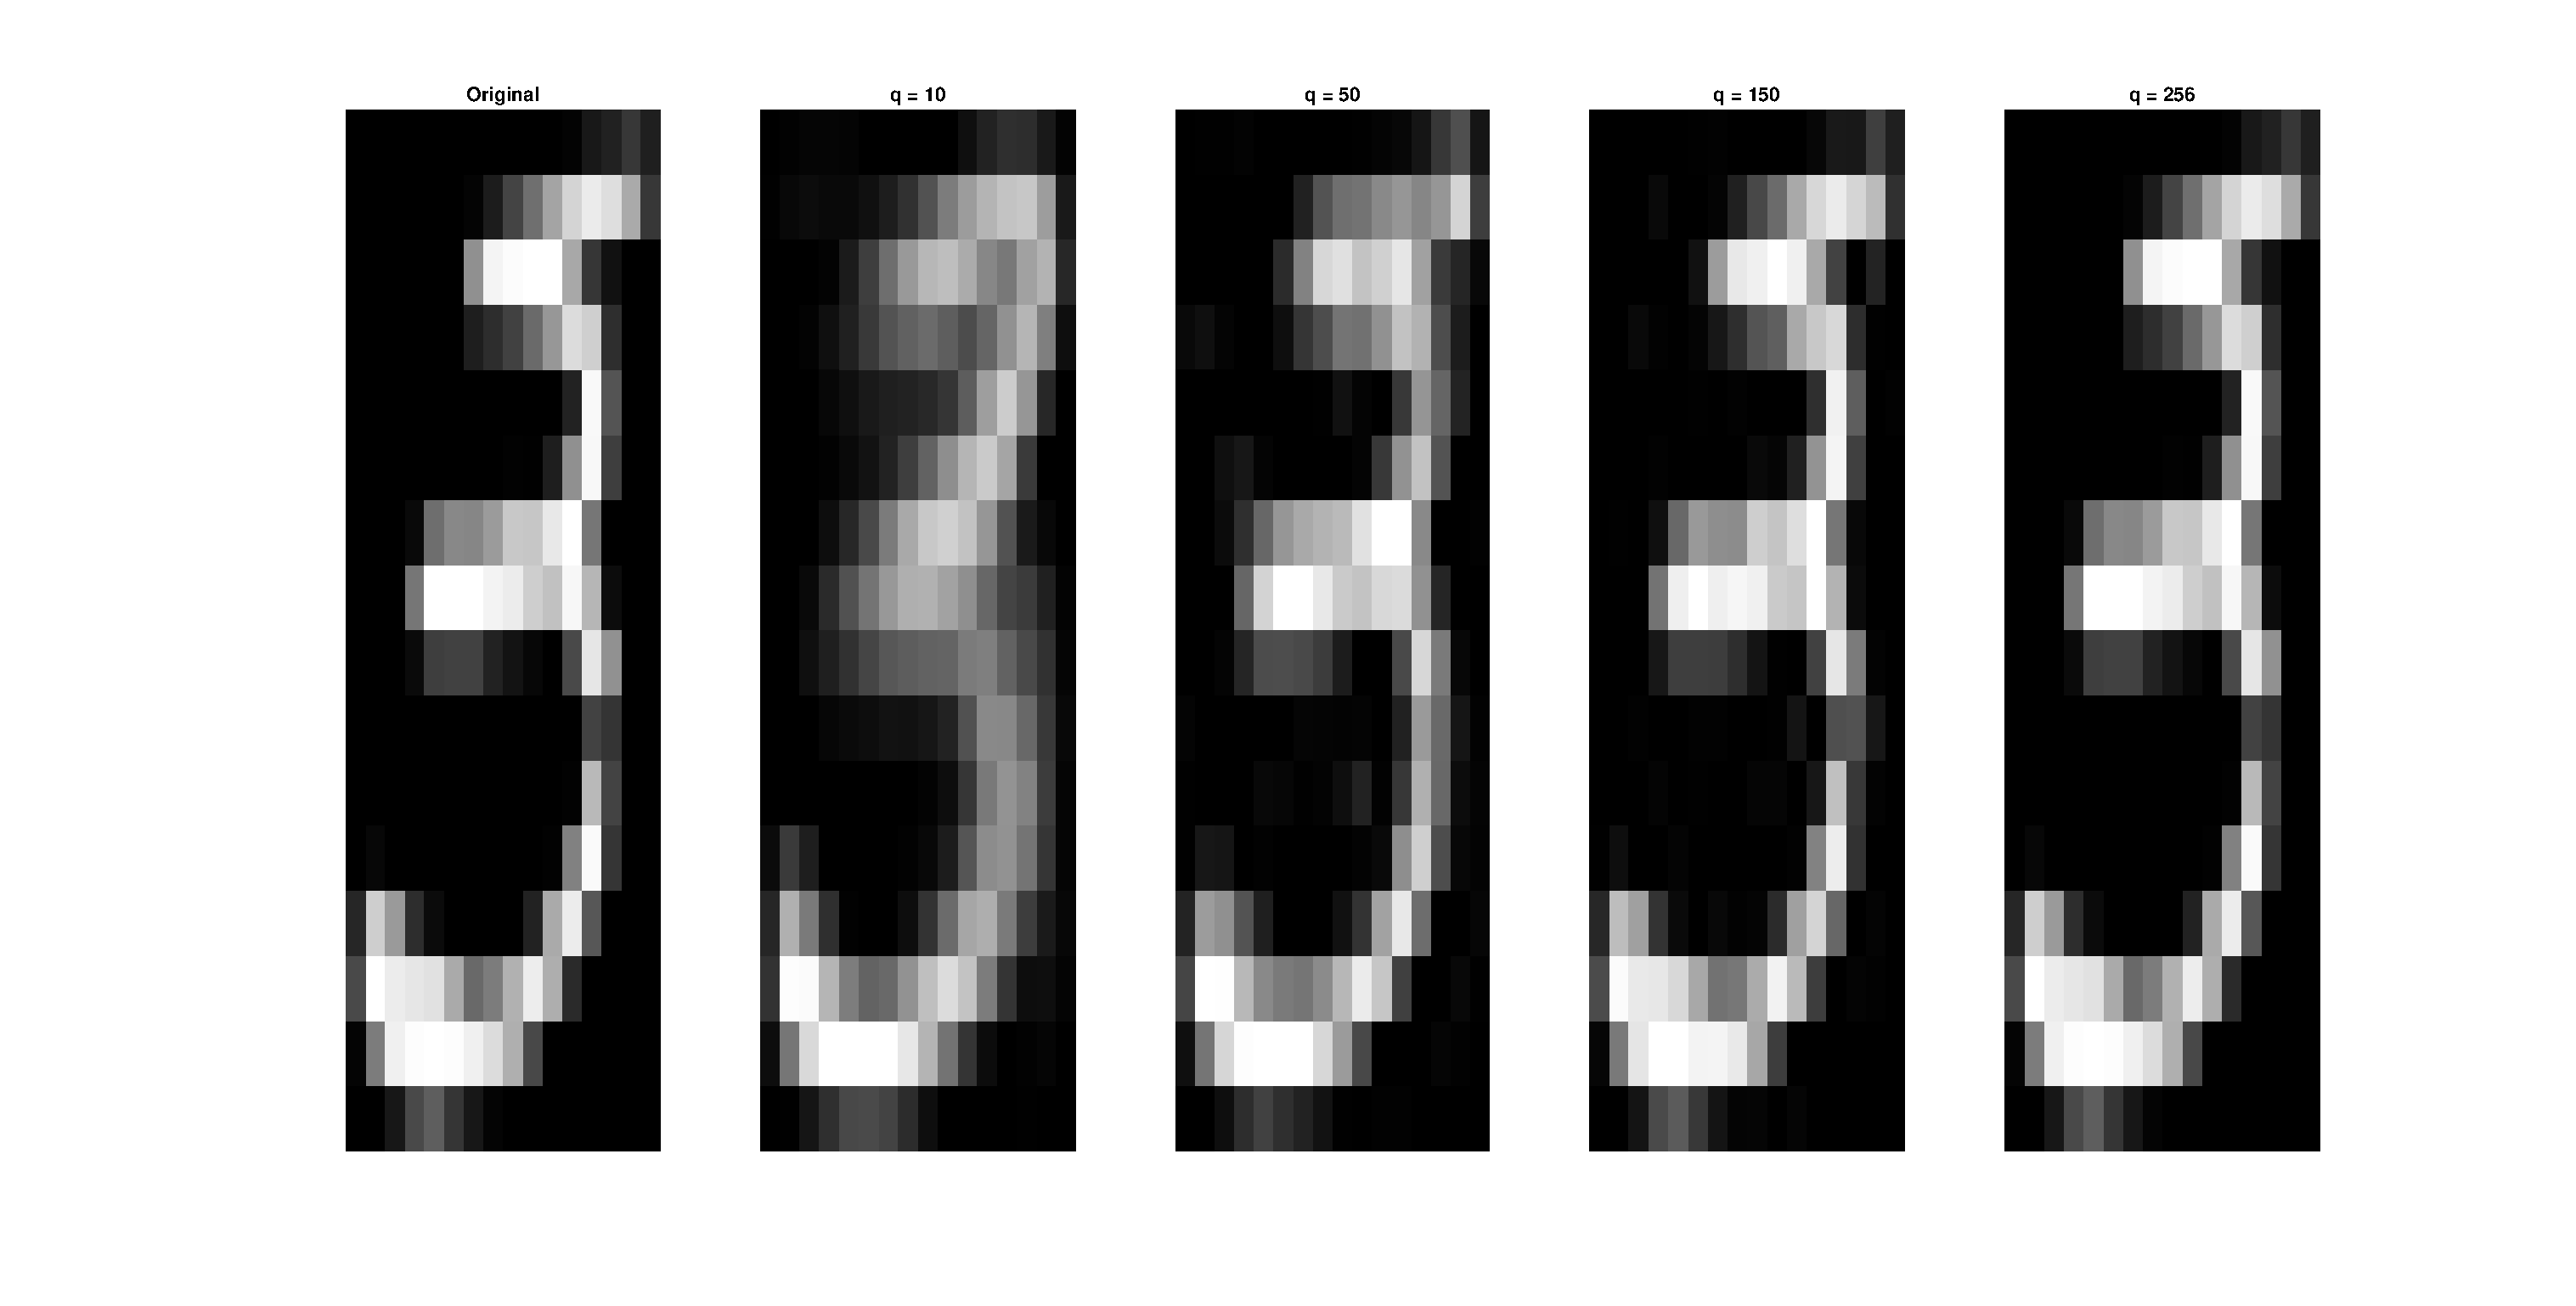
\includegraphics[height = 0.3\textwidth,width = 1.1\textwidth]{Exercise3/Report/pca_dig_2}
		\caption{Original image and reconstructed images with PCA Components [10, 50, 150, 256] - second image to end from left}\label{fig:dig3_2}
	\end{subfigure}%
	\caption{PCA on handwritten digit images of digit 3 }
	\label{fig:dig3}
\end{figure} 
It can be noticed from the figure that for higher values of principal components, the reconstruction becomes more clear as almost all the information is retained. For p=256, we can see that the reconstruction error is zero, as it is the same value as the dimensions of the input data. 


\begin{wrapfigure}{L}{0.45\textwidth}
	\captionsetup{format = hang}
	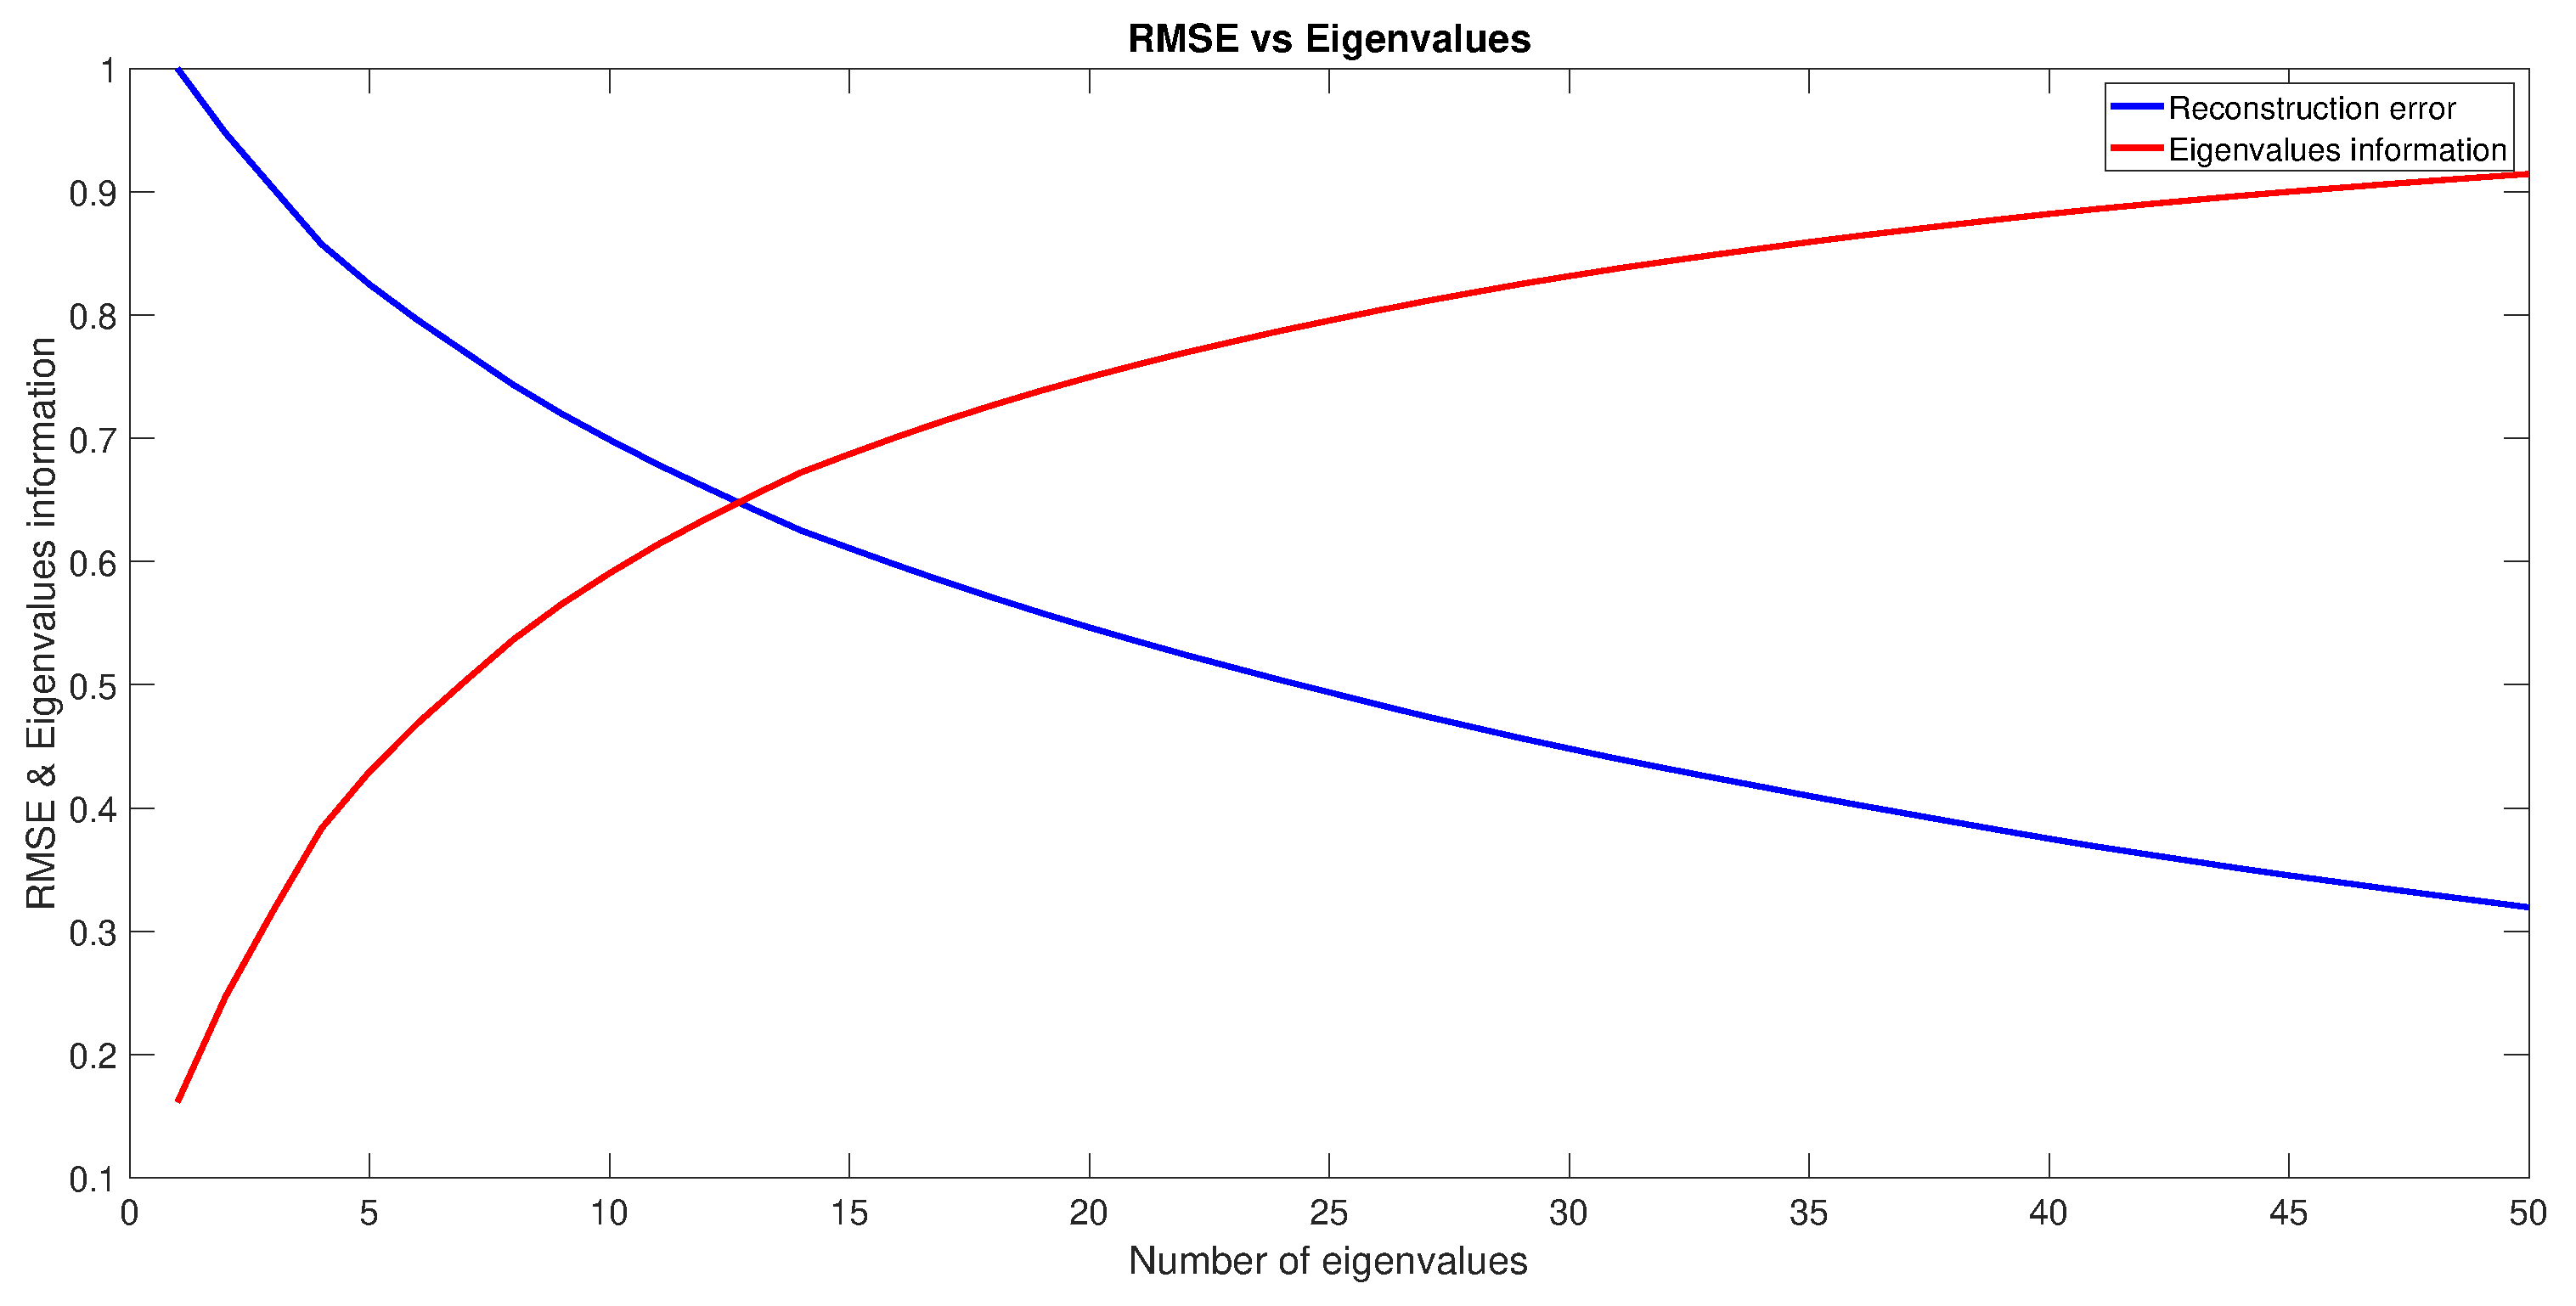
\includegraphics[height = 0.5\textwidth,width = 1.0\textwidth]{Exercise3/Report/pca_eigen}
	\caption{PCA: Reconstruction errors VS Eigen value information}\label{fig:pca_eigen}
\end{wrapfigure}
We then try to analyze the relationship between the reconstruction errors and eigen value information. The plot shown here is for normalized values of errors and cumulative sum of eigen values. From figure \ref{fig:pca_eigen} it can be noticed that the errors and eigen values have an inverse relationship.\\\\
 \newline
\section{Stacked Autoencoders}
A stacked encoder is a neural network with a group of sparse auto encoders where the output of each auto encoder is connected to the consecutive ones. These encoders are trained layer-wise in unsupervised fashion. The output layer of the last encoder can be connected to a softmax layer for the task of classification. We train the stacked encoder for digit classification and some of its results along with the results of a normal neural network is given in the below table.
\begin{table}[!htpb]
	\caption{Performance of stacked autoencoder and neural network models}
	\begin{subtable}{.55\linewidth}
		\centering
		\caption{Stacked Auto-encoder}\label{table:3.1}
		\begin{tabular}{|p{1.2cm}|p{1.2cm}|p{1.2cm}|p{1.2cm}|p{1.6cm}|}
			\hline
			\cellcolor{blue!25}Hidden Layer (HL1)& \cellcolor{blue!25}Hidden Layer (HL2)& \cellcolor{blue!25}Epoch 1(HL1) & \cellcolor{blue!25}Epoch 2(HL2) & \cellcolor{blue!25}Accuracy (\%)\\ \hline
			100 & 50 & 400 & 100 &99.66 \\ \hline
			100 & 50 & 600 & 200 &99 \\ \hline
			100 & 75 & 400 & 100 &\cellcolor{red!25}99.78 \\ \hline	
			150 & 75 & 400 & 100 &95.76 \\ \hline
			150 & 30 & 400 & 100 &99.70 \\ \hline	
			200 & 50 & 400 & 100 &95.42 \\ \hline
			
	\end{tabular}
	\end{subtable}%
	\begin{subtable}{.5\linewidth}
		\centering
		\caption{Neural Network Model}
		\begin{tabular}{|p{3.5cm}|p{2.4cm}|}
			\hline
		\cellcolor{blue!25}	Hidden Layers & \cellcolor{blue!25} Accuracy(\%) \\ \hline
			1 Layer [100] & 97.68 \\ \hline
			2 Layers [100 50] &96.98 \\ \hline
			1 Layer [150] & 96.80 \\ \hline
			2 Layers [150 100] & 95.24 \\ \hline
			1 Layer [250] & 97.26 \\ \hline
			2 Layers [150 30] & 88.72 \\ \hline
		\end{tabular}
	\end{subtable} 
\end{table}\\

The results showed in the table \ref{table:3.1} are obtained by tuning the hyper parameters; number of epochs in hidden layers 1, 2 and number of hidden units in each layer. The stacked auto-encoder with 100 hidden units in hidden layer 1  and 75 hidden units in layer 2 gives better accuracy than other models. Fine tuning has a huge influence on the classification accuracy as the model learns better weights from the encoder layers. On the other hand neural network model does'nt perform as much as the stacked auto-encoder since, the neural network model is trained as a complete network and the encoder is trained layer wise.
\section{Convolutional Neural Networks}
MLP's are not suitable for all neural network applications. MLP's are not translation invariant and using them for object  recognition, classification or any other computer vision tasks can be a bad idea. Convolution neural networks shorty knows as CNN's are popular in most of the computer vision with deep learning tasks. These CNN's are made of convolution blocks that repeatedly applies a filter over the input image to get activation known as feature maps. These features are learnt over various layers of the convolution network and these feature map information is the base for any object detection or classification. In this exercise we first run the \textit{CNNex} script to analyze the working of a CNN. The script uses AlexNet architecture for a classification task on three different classes of objects aeroplane, laptop and a ferry from Caltech101 dataset. The first layer of AlexNet is a input layer that takes an input image of size 224x224x3. The first two layers of the networks uses a max pool layer and the subsequent three layers are connected directly followed by another max pool layer after fifth conv layer. The final three layers are fully connected layers and a softmax layers with 1000 output nodes that gives out probability of the object in a image belonging to a class.

Between every convolution layers there is a ReLU layer that only activates positive inputs and a Normalization  layer that normalizes the previous layer output with its mean and standard  deviation. The output dimensions of every convolution layer is given by  $[\frac{(n+2p-f)}{s}+1] \ X [\frac{(n+2p-f)}{s}+1] \ X n_c$, where $n$ is size of the input, $s$ is stride, $f$ is filter and $n_c$ is number of ouput channels. The below figure shows the feature map of the first layer of the convolution network.
\begin{figure}[!htpb]
	\centering
	\begin{subfigure}[b]{0.5\textwidth}
		\centering
		\captionsetup{width=1\linewidth, format = hang}
		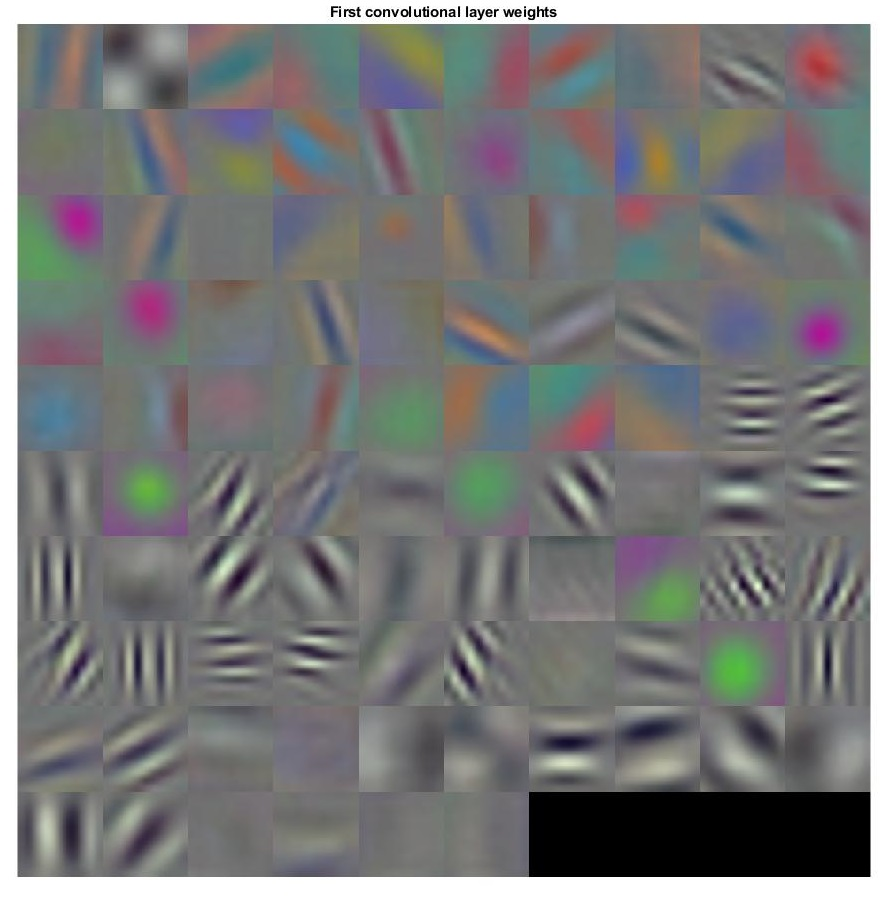
\includegraphics[height = 0.6\textwidth,width = 0.8\textwidth]{Exercise3/Report/conv1}
		\caption{CNN : AlexNet convolution layer 1 weights }\label{fig:conv1}
	\end{subfigure}%
	\begin{subfigure}[b]{0.5\textwidth}
		\centering
		\captionsetup{width=0.8\linewidth, format = hang}
		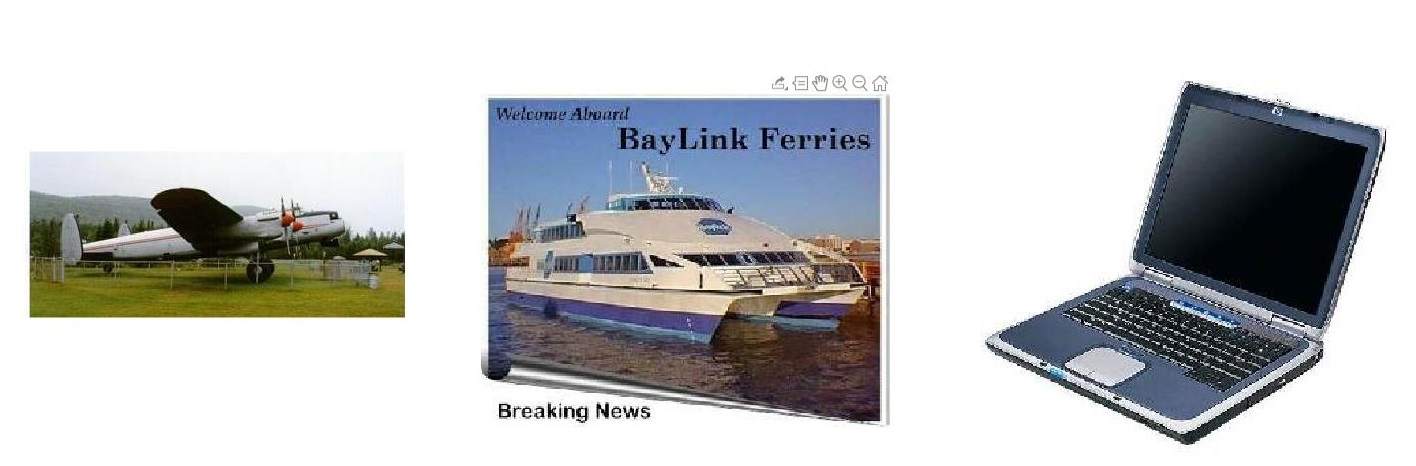
\includegraphics[height = 0.5\textwidth,width = 0.8\textwidth]{Exercise3/Report/conv2}
		\caption{Caltech101 dataset images}\label{fig:conv2}
	\end{subfigure}%
	\caption{ Visualization of CNN weights and datasets}
	\label{fig:cnn}
\end{figure}
From the figure \ref{fig:conv1}, the weights shown for the first layer can learn basic features like edges, strokes, blobs etc. As we go deeper into the layers better features such as shapes are learnt. The first convolution layer in the network uses a filter of size 11x11x3, a stride of 4 and 0 padding layers. Therefore using the output formula as mentioned above we get the output size of first convolution layer as  55x55x96. ReLU and normalization layers do not alter the output dimensions. The output after the max pool layer is given by $[\frac{n-P_s}{S}+1]$, where $P_s$ is the pool size. The network uses a max pool size of 3x3 and a stride of 2. Therefore, the size of the layer after first max pooling is given by (55-3/2)+1 = 27x27x96. Similarly, the output after fifth convolution layer and max pooling is obtained as 6x6x256. The final fully connected layers have a size of 4096 and the softmax layer as 1000(number of classes in our case) compared to input dimensions 227x227x227=154,587 as the image size gets  down sampled over the convolution and max pool layers. 

CNN's are better at feature extractions than fully connected layers. The number of weights required for a CNN training gets reduced by down sampling over the convolution layers which is not the case with only fully connected networks. Due to the large number of parameters to be tuned in the network, FCN's can   take longer durations for training and chances of over-fitting is also high.

We then run the script \textit{CNNDigits} to evaluate the classification capabilities of a CNN. We train and test the models by changing various layers. Some of the results for the same are shown in the table \ref{table:3.2}. The trained is done on GPU, therefore the training time for all the architectures that are experimented is less than 40 secs. It can be noticed that the architecture with convolution layer1  with 32 filters and size 5, convolution layer2 with 64 filters and size 5 gives maximum accuracy of 98.24. The architecture with 4 convolution layers and filter size 3 couldn't give better performance than the one with 2 layers and filter size 5. From these results it can be said that the choice of convolution layers and filters influence a CNN's performance.
 
\begin{table}[!htpb]
	\centering
	\begin{tabular}[t]{|>{\centering}p{6 cm}|p{4.8cm}|p{5.1cm}|}
		
		\cellcolor{blue!25}CNN Architecture Layers & \cellcolor{blue!25} Training Accuracy Graph& \cellcolor{blue!25} Training time and accuracy \\ \hline
		
			&&\\
		\vspace*{-2.8cm}
	convolution2dLayer(5,12);
	reluLayer;
	
	maxPooling2dLayer(2,'Stride',2);
	
	convolution2dLayer(5,24);
	reluLayer &  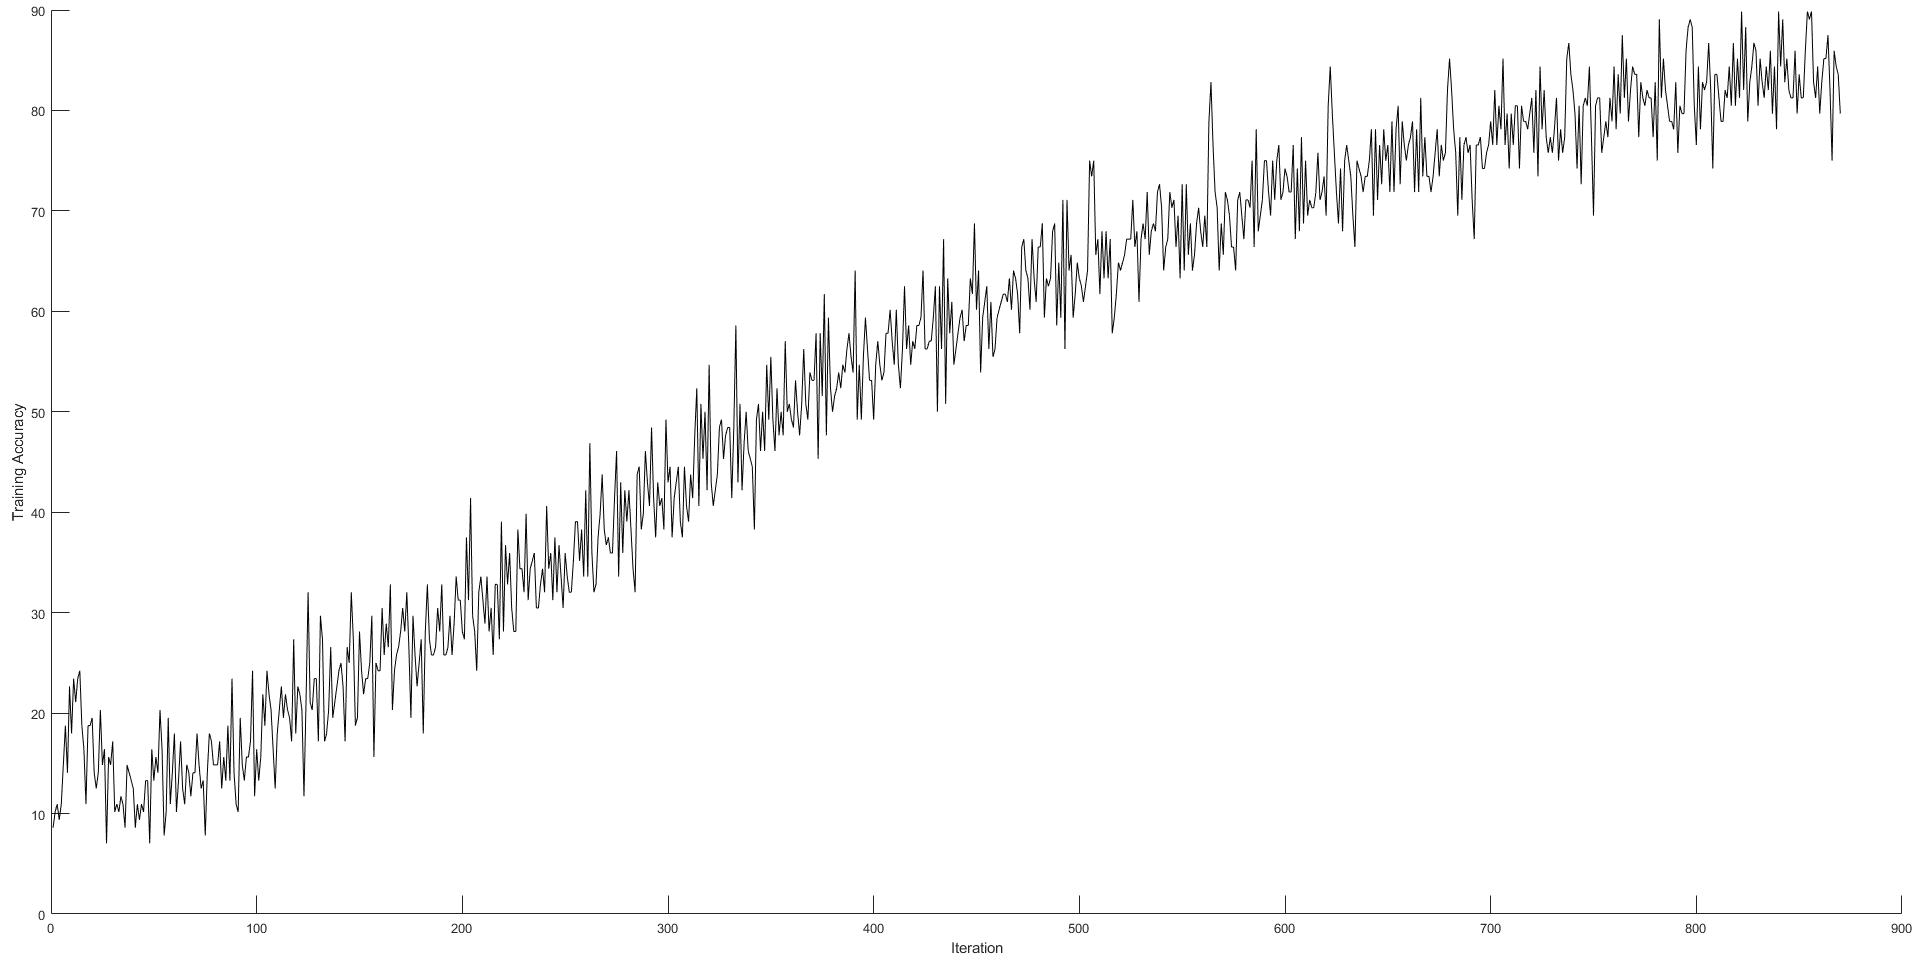
\includegraphics[height=3cm, width=4.4cm]{Exercise3/Report/accuracy_1_82} &  Accuracy = 82.08 \newline Time elapsed = 25.611191 secs\\ \hline
		
		&&\\
		\vspace*{-2.8cm}
	convolution2dLayer(3,32); reluLayer ; 	maxPooling2dLayer(2,'Stride',2); convolution2dLayer(3,64); reluLayer; maxPooling2dLayer(2,'Stride',2); convolution2dLayer(3,128); reluLayer;	
	convolution2dLayer(3,256);	reluLayer&  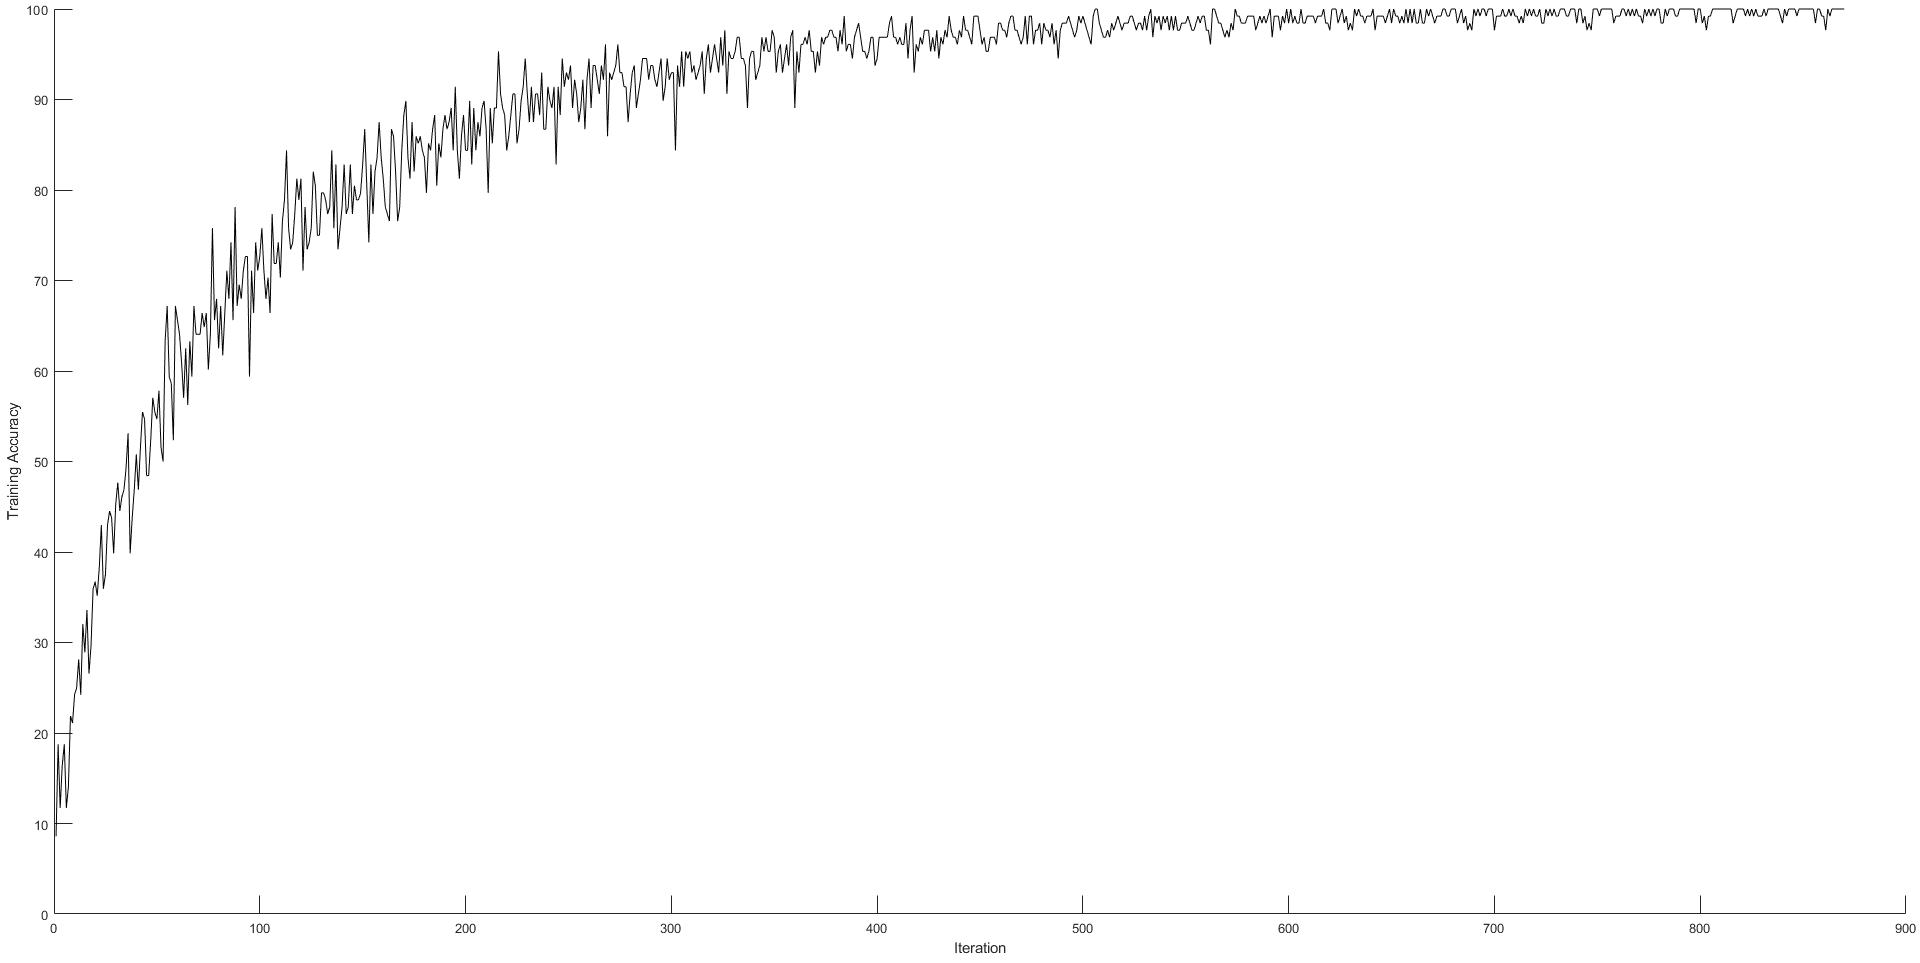
\includegraphics[height=3cm, width=4.4cm]{Exercise3/Report/accuracy_5_97_60} &  Accuracy = 97.60 \newline Time elapsed = 37.527818 secs\\ \hline
		
		&&\cellcolor{green!25} \\
		\vspace*{-2.8cm}
		convolution2dLayer(5,32);
		reluLayer;
		
		maxPooling2dLayer(2,'Stride',2);
		
		convolution2dLayer(5,64);
		reluLayer   &  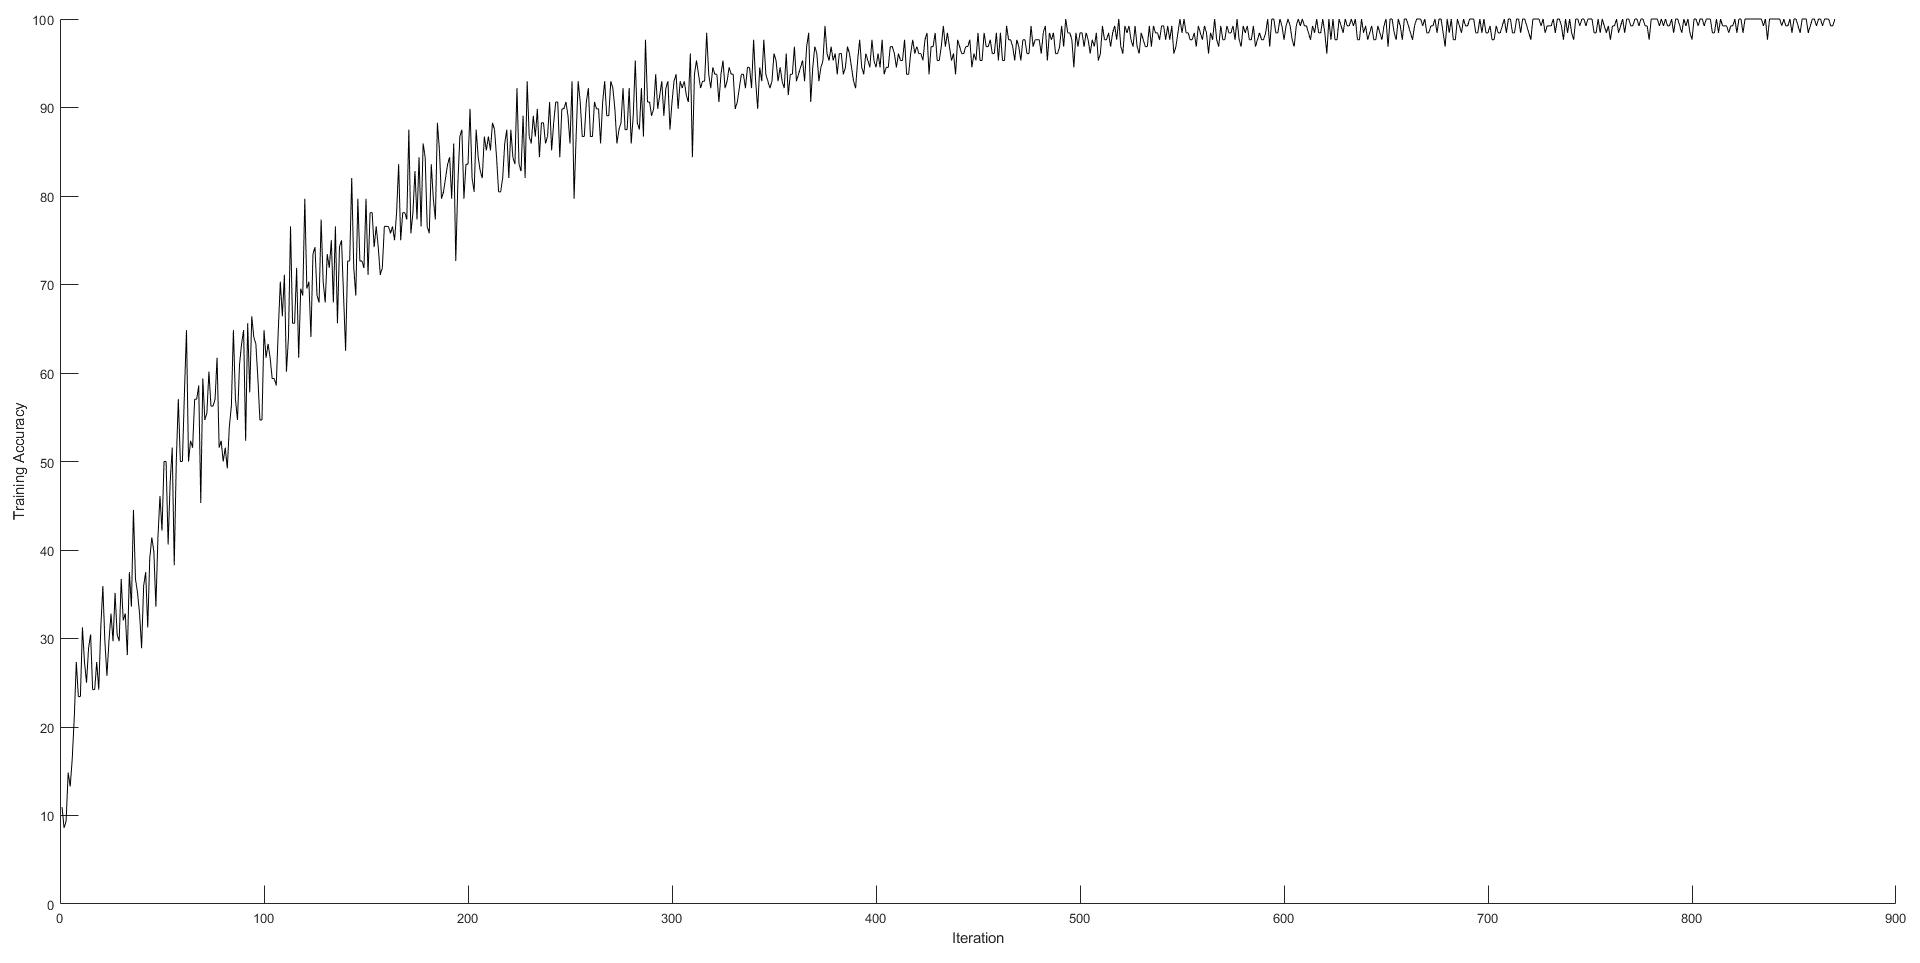
\includegraphics[height=3cm, width=4.4cm]{Exercise3/Report/accuracy_3_97_68} &  \cellcolor{green!25} Accuracy = 98.24 \newline Time elapsed = 33.306200 secs\\ \hline
		
		&&\\
		\vspace*{-2.8cm}
		convolution2dLayer(7,32); reluLayer ; 	maxPooling2dLayer(2,'Stride',2); convolution2dLayer(7,64); reluLayer; &  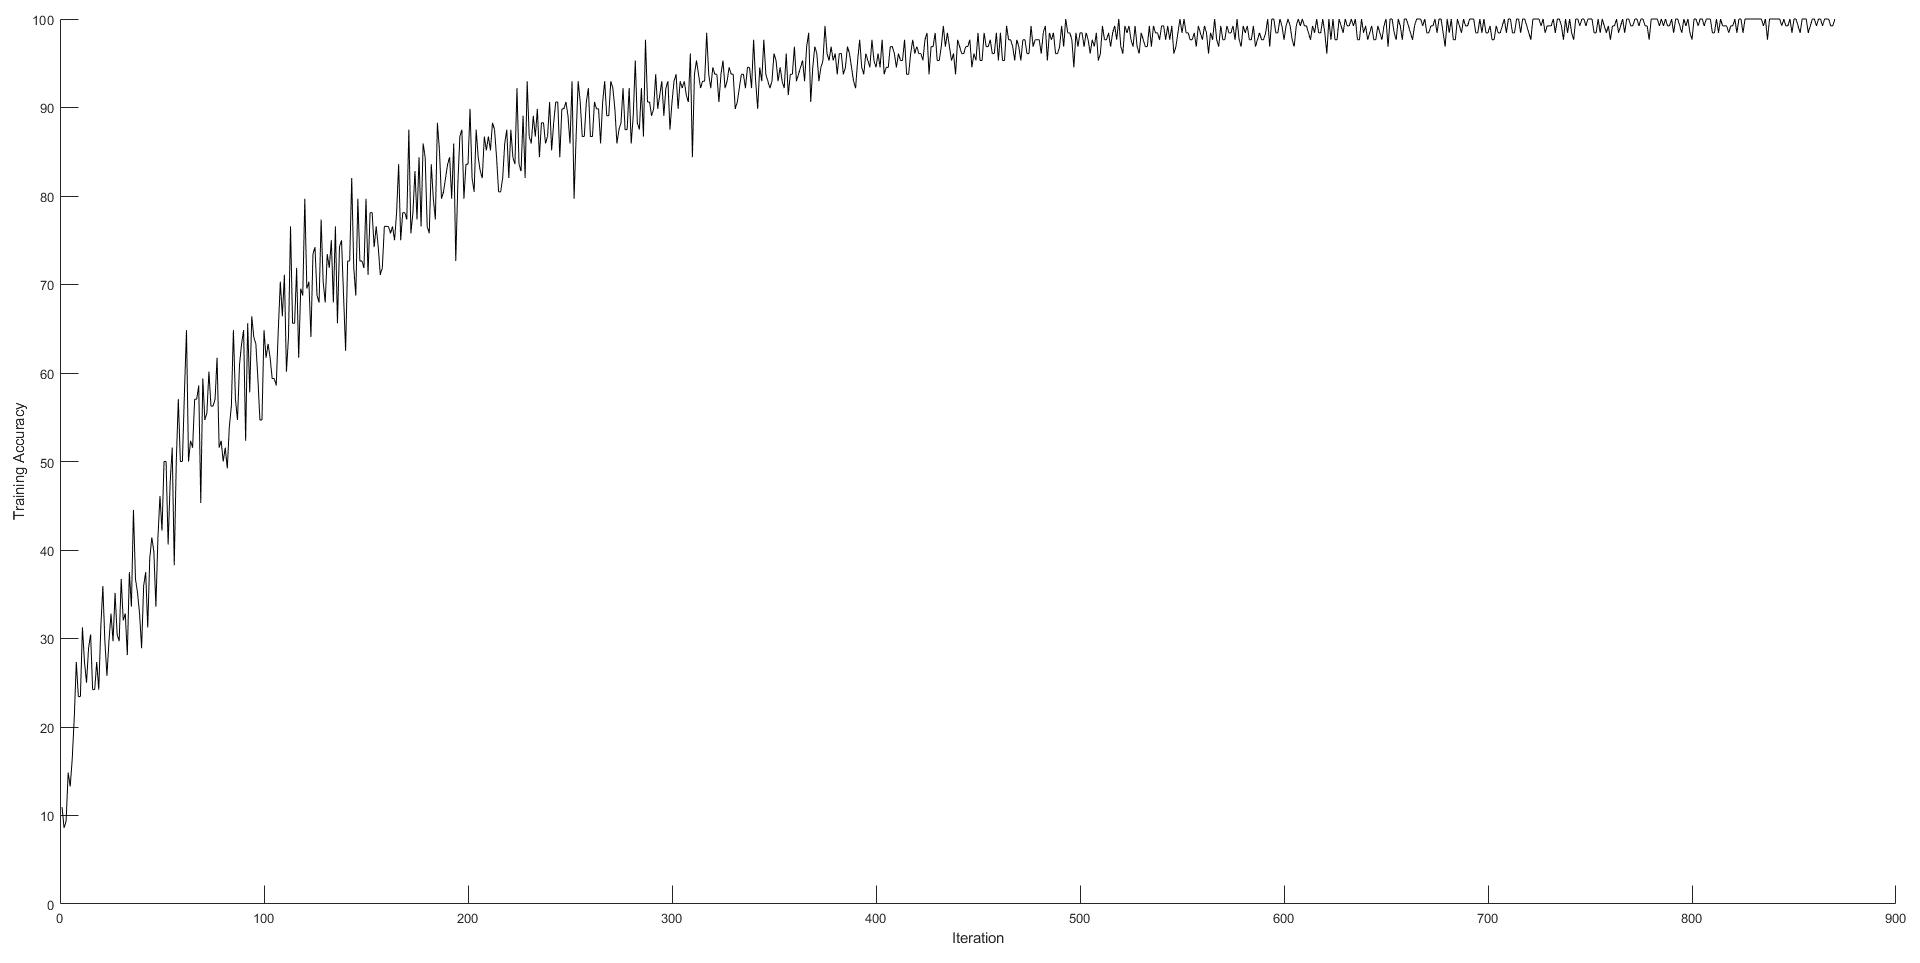
\includegraphics[height=3cm, width=4.4cm]{Exercise3/Report/accuracy_3_97_68} &  Accuracy = 97.68 \newline Time elapsed = 27.847668 secs\\ \hline
		
		
	\end{tabular}
	
	\captionsetup{format = hang}
	\caption{Performance of a CNN in classifying digits dataset for various architectures}
	\label{table:3.2}
\end{table}